\documentclass[../TDE4-E5.tex]{subfiles}%

\begin{document}
\section[s]"2"{RLC échelon montant}

\begin{center}
	Indiquer la ou les bonnes réponses en justifiant tout votre raisonnement.
\end{center}

On considère un circuit RLC série, alimenté par une source idéale de tension de
force électromotrice $E$ constante comme schématisé ci-contre. Le condensateur
peut être court-circuité lorsque l'interrupteur K est fermé. On note $i(t)$
l'intensité du courant qui traverse la bobine et $u_C(t)$ la tension aux bornes
du condensateur C.

\begin{figure}[htbp]
	\centering
	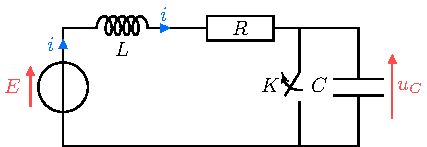
\includegraphics[width=.5\linewidth]{rlc_montant_switch}
\end{figure}

Le condensateur est mis en court-circuit par un interrupteur K depuis une durée
suffisamment longue, pour que le régime permanent soit établi. À l'instant pris
comme origine des temps, on ouvre l'interrupteur K.

\QR{Que valent l'intensité $i\left(0^+\right)$ et la tension $u_C(0^+)$ à
	l'instant $t=0^+$, succédant immédiatement à l'ouverture de l'interrupteur K~?
	Justifier tout votre raisonnement.
	\begin{tasks}[label=\protect\fbox{\Alph*}, label-width=4ex](4)
		\task $i\left(0^+\right)=0$
		\task $i\left(0^+\right)=\frac{E}{R}$
		\task $u_C\left(0^+\right)=0$
		\task $u_C\left(0^+\right)=E$
	\end{tasks}%
}{%
	Intéressons-nous d'abord au circuit à $t<0$. L'interrupteur est alors fermé si
	bien que $u_C$ est une tension aux bornes d'un fil donc
	\smallbreak
	\centers{$u_C\left(t=0^-\right)=0$}
	\smallbreak
	De plus, le condensateur assure la continuité de la tension à ses bornes,
	donc
	\smallbreak
	\centers{$u_C\left(t=0^+\right)=u_C\left(t=0^-\right)=0$}
	\smallbreak
	Par ailleurs en régime permanent constant, on sait que la bobine est
	équivalente à un interrupteur fermé (un fil). Si bien que le circuit est alors
	équivalent à uniquement la résistance $R$ en série avec la source idéale de
	fem $E$. Ainsi d'après la loi de Pouillet,
	\smallbreak
	\centers{$i\left(t=0^-\right)=E/R$}
	\smallbreak
	De plus, la bobine assure la continuité de l'intensité qui la traverse, donc
	\smallbreak
	\centers{$i\left(t=0^+\right)=i\left(t=0^-\right)=\frac{E}{R}$}
	\smallbreak
	Réponses B et C.
}

\QR{Etablir l'équation différentielle vérifiée par $u_C(t)$ pour $t>0$.
	On la mettra sous forme canonique en introduisant la pulsation propre $\w_0$ et le facteur de qualité $Q$~:
	\smallbreak
	\centers{$\frac{\dd^2 u_C(t) }{\dd t^2}+\frac{\w_0}{Q} \frac{\dd u_C(t) }{\dd
				t}+ \w_0^2 u_C(t) = \alpha$}
	\smallbreak
	Exprimer $\w_0$ et $Q$.
	\begin{tasks}[label=\protect\fbox{\Alph*}, label-width=4ex](4)
		\task $\w_0=\frac{1}{\sqrt{LC}}$
		\task $\w_0=\frac{1}{LC}$
		\task $Q=R\sqrt{\frac{L}{C}}$
		\task $Q=\frac{1}{R}\sqrt{\frac{L}{C}}$
	\end{tasks}
}{
	On se place après l'ouverture de l'interrupteur ($t>0$). On a alors un circuit
	RLC série pour lequel on cherche à établir l'équation différentielle du second
	ordre sur la variable $u_C(t)$. Appliquons la loi des mailles en
	notant $u_R$ et $u_L$ les tensions respectivement aux bornes du résistor et de
	la bobine.
	\begin{DispWithArrows*}
		u_L + u_R = u_C &= E
		\Arrow{$u_L = L \dv{i}{t}$\\et $u_R = Ri$}
		\\\Lra
		L \dv{i}{t} + Ri + u_C &= E
		\Arrow{$i = C \dv{u_C}{t}$}
		\\\Lra
		LC \dv[2]{u_C}{t} + RC \dv{u_C}{t} + u_C                   &= E
		\Arrow{forme\\canonique}
		\\
		\Lra \dv[2]{u_C}{t} + \frac{R}{L} \dv{u_C}{t} + \frac{1}{LC}u_C &=
		\frac{E}{LC}
	\end{DispWithArrows*}
	\leftcenters{Par identification, on a alors :} {${\w_0}^2=\frac{1}{LC}$}
	\smallbreak
	\leftcenters{ Ainsi }{$\w_0=\frac{1}{\sqrt{LC}}\quad  \text{et} \quad \frac{\w_0}{Q}=\frac{R}{L}$}
	\smallbreak
	\leftcenters{Soit}{$Q=\frac{L\w_0}{R}=\frac{L}{R}\frac{1}{\sqrt{LC}}=\frac{1}{R}\sqrt{\frac{L}{C}}$}
	\medskip
	Réponses A et D.
}

\QR{Exprimer $\alpha$.
\begin{tasks}[label=\protect\fbox{\Alph*}, label-width=4ex](4)
	\task $\alpha=0$
	\task $\alpha=E$
	\task $\alpha=QE$
	\task $\alpha= {\w_0}^2 \, E$
\end{tasks}
}{
En poursuivant l'identification on constate encore que :
\smallbreak
\centers{$\alpha=\frac{E}{LC}={\w_0}^2E$}
\medskip
Réponse D.
}

\QR{Que peut-on affirmer concernant le facteur de qualité ?
	\begin{tasks}[label=\protect\fbox{\Alph*}, label-width=4ex]
		\task La durée du régime transitoire est la plus brève lorsque $Q=2$.
		\task La durée du régime transitoire est la plus brève lorsque $Q=1/2$.
		\task Plus la valeur de l'inductance est élevée, plus le facteur de qualité est faible.
		\task Plus la valeur de la capacité est élevée, plus le facteur de qualité est faible.
	\end{tasks}
}{
	La durée du régime transitoire est la plus brève lorsque le système a une
	évolution pseudo-périodique avec un très faible dépassement, soit pour un
	$Q>1/2$ (précisément, c'est pour $Q=0,72$). Aucune des deux premières
	réponses A ou B n'est juste. Notez en revanche que pour $Q=1/2$, on a le
	transitoire le plus bref sans dépassement. Par ailleurs, le facteur de
	qualité s'écrivant
	\smallbreak
	\centers{ $Q=\frac{1}{R}\sqrt{\frac{L}{C}}$ }
	\smallbreak
	Une inductance élevée induira un facteur de qualité grand tandis qu'une capacité élevée conduira à un facteur de qualité petit.
	\medskip
	Réponse D.
}

Dans la suite, on considère que la bobine possède une inductance L=50 mH et que
la capacité du condensateur vaut $C =\SI{20}{\mu F}$. On souhaite obtenir un
facteur de qualité $Q=10$.

\QR{Calculer la valeur à donner à la résistance $R$ du résistor.
	\begin{tasks}[label=\protect\fbox{\Alph*}, label-width=4ex](4)
		\task $R=\SI{0,002}{\ohm}$
		\task $R=\SI{0,02}{\ohm}$
		\task $R=\SI{5}{\ohm}$
		\task $R=\SI{500}{\ohm}$
	\end{tasks}
}{
	On cherche la valeur de $R$ pour obtenir $Q=10$ à $L$ et $C$ fixé.
	On isole alors $R$ dans l'expression de $Q$ :
	\smallbreak
	\centers{$R=\frac{1}{Q}\sqrt{\frac{L}{C}}=\frac{1}{10}\sqrt{\frac{50\times{10}^{-3}}{20\times{10}^{-6}}}=\SI{5}{\ohm}$}
	\medskip
	Réponse C.
}

\enonce{On admet alors que la tension aux bornes du condensateur évolue selon :
\[
	u_C(t)=\exp(- \frac{t}{\tau})\left[A\cos{\left(\Wt\right)+B\sin{\left(\Wt\right)}}\right]+u_{C,p}
\]
}

\QR{Exprimer $\tau$ en fonction de $\w_0$ et $Q$. Justifier tout votre
raisonnement.
\begin{tasks}[label=\protect\fbox{\Alph*}, label-width=4ex](4)
	\task $\tau=\frac{\w_0}{2Q}$
	\task $\tau=\frac{2Q}{\w_0}$
	\task $\tau=\frac{\w_0}{Q}$
	\task $\tau=\frac{Q}{\w_0}$
\end{tasks}
}{
Le polynôme caractéristique associé à l'équation différentielle canonique
s'écrit :
\smallbreak
\centers{$s^2+\frac{\w_0}{Q}s+{\w_0}^2=0$}
\smallbreak
\leftcenters{De discriminant :} {$\Delta=\left(\frac{\w_0}{Q}\right)^2-4{\w_0}^2={{\w}_0}^2\left(\frac{1}{Q^2}-4\right)<0 \quad \text{car} \quad Q=10>\frac{1}{2}$}
\smallbreak
Les racines s'écrivent donc, avec  $j^2=-1$,
\smallbreak
\centers{$r_\pm=-\frac{\w_0}{2Q}\pm j \frac{\sqrt{-\Delta}}{2} =-\frac{\w_0}{2Q}\pm j \w_0 \sqrt{1-\frac{1}{4Q^2}}$}
\smallbreak
Que l'on peut identifier avec la forme des racines proposée par l'énoncé pour être en cohérence avec l'expression de $u_C\left(t\right)$ :
\smallbreak
\centers{ $r_\pm=-\frac{1}{\tau}\pm j\W$ }
\smallbreak
\leftcenters{Ainsi, par identification,}             {$\tau=\frac{2Q}{\w_0}$}
\medskip
Réponse B.
}

\QR{Exprimer la pseudo-pulsation $\W$ en fonction de $\w_0$ et $Q$. Justifier
	tout votre raisonnement.
	\begin{tasks}[label=\protect\fbox{\Alph*}, label-width=4ex,
			item-indent=-1em, column-sep=8em](4)
		\task $\W=\w_0\sqrt{1-\frac{1}{4Q^2}}$
		\task $\W=\w_0\sqrt{\frac{1}{4Q^2 }-1}$
		\task $\W=\w_0\left(1+\frac{1}{4Q^2}\right)^{1/2}$
		\task $\W=\frac{\w_0}{\sqrt{1-\frac{1}{4Q^2}}}$
	\end{tasks}
}{
	\leftcenters{De même, par identification, }{$\W=\frac{\sqrt{-\Delta}}{2}=\w_0\sqrt{1-\frac{1}{4Q^2}}$}
	\medskip
	Réponse A.
}

\QR{Exprimer $u_{C,p}$ en fonction de $E$. Justifier tout votre raisonnement.
\begin{tasks}[label=\protect\fbox{\Alph*}, label-width=4ex](4)
	\task $u_{C,p}=E$
	\task $u_{C,p}=0$
	\task $u_{C,p}=\w_0{}^2 E$
	\task $u_{C,p}=2E$
\end{tasks}
}{
$u_{C,p}$ est la solution particulière de l'équation différentielle. On peut la
chercher sous la forme d'une constante. Soit, en l'injectant dans l'équation
différentielle :
\smallbreak
$\frac{\dd^2u_{C,p}}{\dd t^2}+\frac{R}{L}\frac{\dd u_{C,p}}{\dd t}+\frac{u_{C,p}}{LC}=\frac{E}{LC}$
\smallbreak
\leftcenters{D'où : }{$0+0+\frac{u_{C,p}}{LC}=\frac{E}{LC} \quad \text{d'où} \quad u_{C,p}=E$}
\medskip
Réponse A.
}

\QR{Exprimer A. Justifier tout votre raisonnement.
	\begin{tasks}[label=\protect\fbox{\Alph*}, label-width=4ex](4)
		\task $A=E$
		\task $A=-E$
		\task $A=0$
		\task $A=E/2$
	\end{tasks}
}{
	Exprimons les constantes d'intégration $A$ et $B$ à l'aide des conditions initiales déterminées à la question 1 :
	\smallbreak
	\centers{$u_C\left(t=0^+\right)=0=\exp(-0/\tau)\left[A\cos{\left(0\right)}+B\sin{\left(0\right)}\right]+E$}
	\smallbreak
	\leftcenters{ Ainsi :}{ $A=-E$}
	\medskip
	Réponse B.
}

\QR{Exprimer B. Justifier tout votre raisonnement.
	\begin{tasks}[label=\protect\fbox{\Alph*}, label-width=4ex,
			item-indent=2.5em, column-sep=4em](4)
		\task $B=\frac{E}{\W}\pa{\frac{1}{RC}-\frac{1}{\tau}}$
		\task $B=\frac{E}{{RC\w}_a}$
		\task $B=0$
		\task $B=\frac{E}{{\tau \w}_a}$
	\end{tasks}
}{
	D'après Q1, on a aussi $i\left(t=0^+\right)=E/R$.
	Or, la loi courant tension aux bornes du condensateur permet d'écrire que :
	\smallbreak
	\centers{${\dot{u}}_C\left(t=0^+\right)=\frac{i\left(t=0^+\right)}{C}=\frac{E}{RC}$}
	\smallbreak
	Dérivons $u_C\left(t\right)$. Il vient
	\smallbreak
	${\dot{u}}_C\left(t\right)=-\frac{1}{\tau}exp\left(-t/\tau\right)\left[A\cos{\left(\Wt\right)}+B\sin{\left(\Wt\right)}\right]+\W\times \exp\left(-t/\tau\right)\left[-A\sin{\left(\Wt\right)}+B\cos{\left(\Wt\right)}\right]$
	\smallbreak
	\leftcenters{Soit, en $t=0$,}
	{ ${\dot{u}}_C\left(t=0^+\right)=-\frac{A}{\tau}+\W B=\frac{E}{RC}$}
	\smallbreak
	\leftcenters{ Ainsi }{$\W B=\frac{E}{RC}+\frac{A}{\tau}$}
	\smallbreak
	\leftcenters{D'où, avec $A=-E$, }
	{ $B=\frac{E}{\W}\left(\frac{1}{RC}-\frac{1}{\tau}\right)$}
	\smallbreak
	\medskip
	Réponse A.
	\bigskip
	\leftcenters{De plus} {$\tau=\frac{2Q}{\w_0}=\frac{2}{R}\sqrt{\frac{L}{R}}\times\sqrt{LC}=\frac{2L}{R}$}
	\smallbreak
	Donc $\tau$ ne s'exprime pas en fonction de $R$ et $C$ uniquement. Ainsi, la
	réponse B est fausse. De même, $RC$ ne peut pas s'exprimer simplement en
	fonction de $\tau$ donc la réponse D est fausse.
}

\end{document}
